%!TEX root = ../dokumentation.tex


\chapter{Validierung des Systems}

Nachdem das Aufnehmen und Darstellen von Räumen funktioniert, wird die Genauigkeit des Systems untersucht. Zudem werden Versuche zu verschiedenen Auflösungen und unterschiedlicher Sensoren durchgeführt.  


\section{Genauigkeit des Systems}

Um die Genauigkeit des Systems zu überprüfen, wird ein Raum mit dem Lidar-System vermessen. Zudem wird der Raum händisch vermessen und der Grundriss mit der Software "Sweet Home 3D" erstellt. Anschließend wird die 3D-Darstellung mit dem Grundriss des Raumes und weiterer markanter Gegenstände verglichen.
Bei dem Raum handelt es sich um einen Flur mit vielen Ecken, Türen und Gegenständen. Dadurch erhält man viele verschiedene Maße, die überprüft werden können. Der Grundriss des Raumes ist in Bild ... dargestellt. Alle weiteren Maße des Raumes können direkt in der Software abgerufen werden.

\begin{figure}[H]
	\centering
	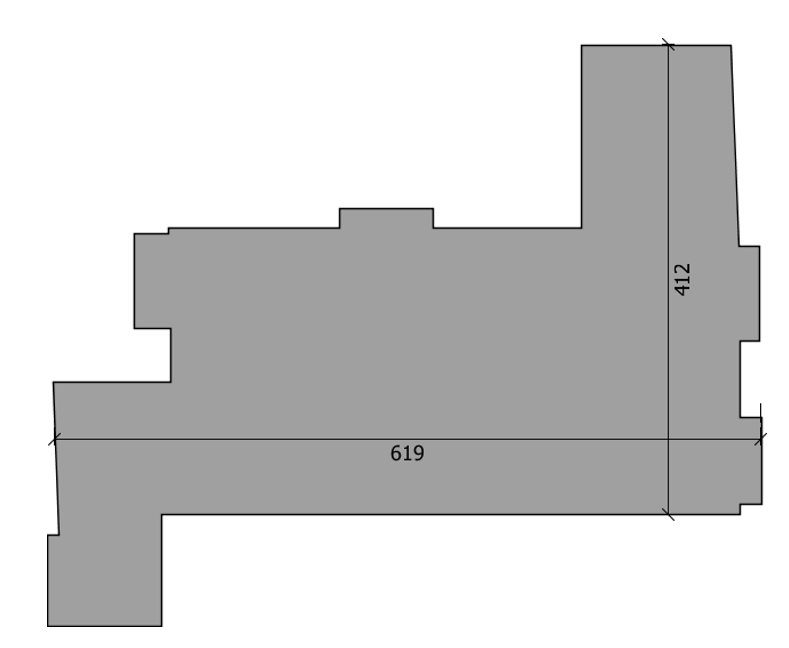
\includegraphics[width=0.7\textwidth]{images/Validierung/Grundriss}
	\caption{Grundriss des Testraums}
	\label{grundriss}
\end{figure}


Das Lidar-System wird im Raum aufgestellt, die Position ist annähernd mittig und wird zudem ausgemessen und in der Software eingetragen. Durch die Funktionsweise von Lidar Sensoren entstehen Schatten. So können beispielsweise Konturen hinter einer Wand, die die Lichtstraheln reflektiert nicht detektiert werden. Diese Schatten werden ebenfalls im Grundriss eingezeichnet, um den Vergleich besser durchführen zu können. Die weißen Stellen innerhalb des Grundrisses in Abbildung ... stellen diese Schatten dar.

\begin{figure}[H]
	\centering
	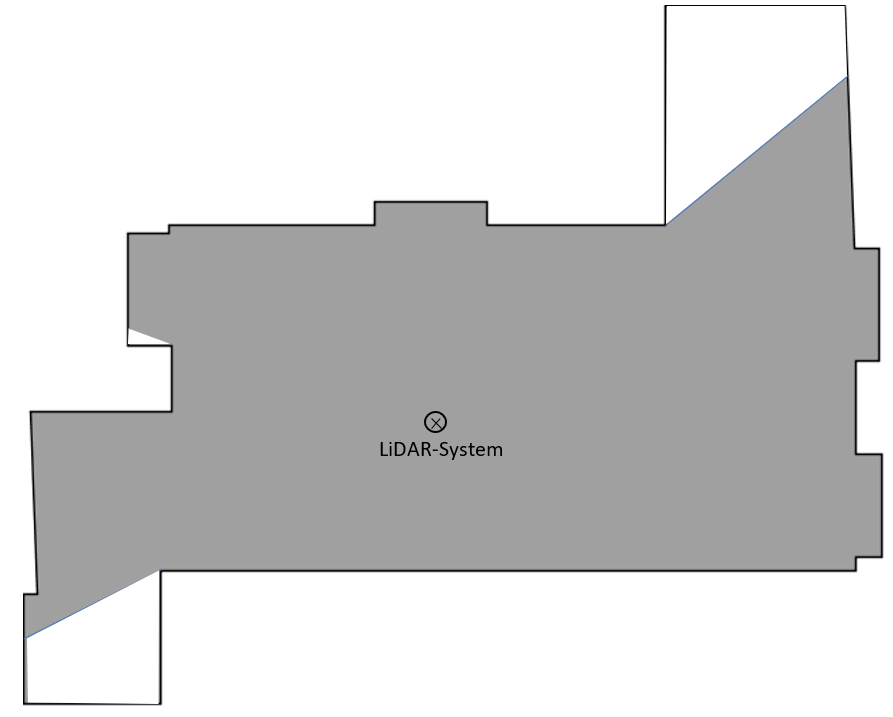
\includegraphics[width=0.7\textwidth]{images/Validierung/MitSchatten}
	\caption{Grundriss des Testraums}
	\label{grundrssmitschatte}
\end{figure}


Zum Vergleich wird nun der Grundriss benötigt, den das Lidar-System erstellt hat. Dazu wird die 3D Darstellung nur in z-Richtung betrachtet. Man erhält eine Vogelperpektive des Raumes, bei dem der Grundriss auszumachen ist. 

\begin{figure}[H]
	\centering
	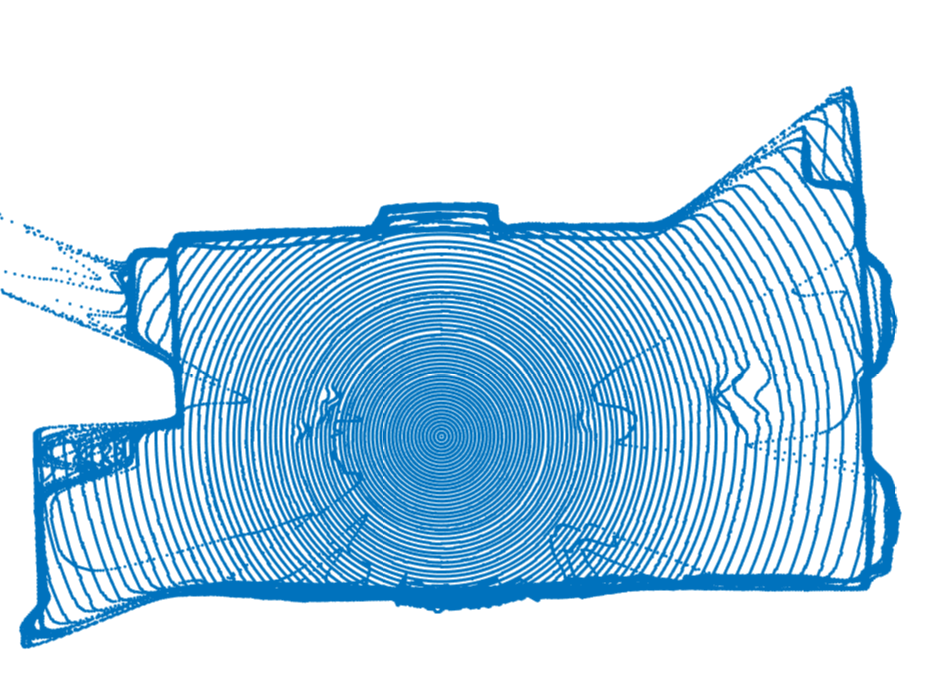
\includegraphics[width=0.7\textwidth]{images/Validierung/Vogelperspektive}
	\caption{Vogelperspektive des Testraums}
	\label{vogelperspektive}
\end{figure}


Zum grafischen Vergleich werden manuell erstellter Grundriss und die Vogelperspektive des Testraums mit einem Bildbearbeitungsprogramm im gleichen Maßstab übereinander gelegt.

\begin{figure}[H]
	\centering
	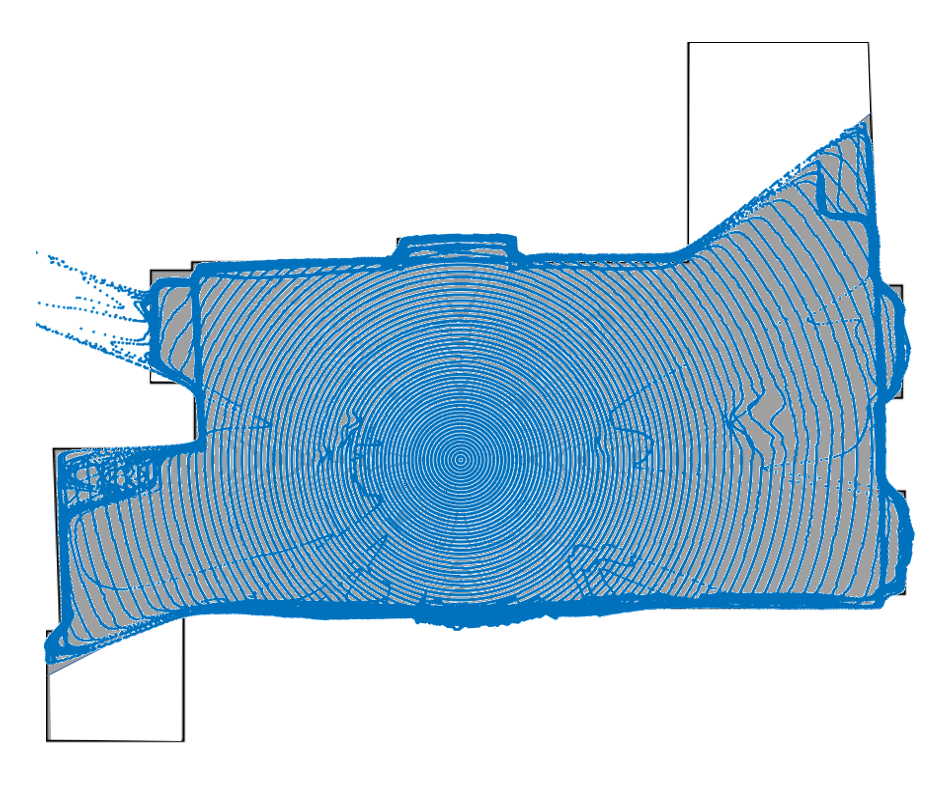
\includegraphics[width=0.7\textwidth]{images/Validierung/uebereinander}
	\caption{Grafischer Vergleich der Grundrisse}
	\label{uebereinander}
\end{figure}


-- Was kann man sehn?
--nur 2 Linien nehemn

-- Linien an Seite raus weil Glas

-- Höhe wird überprüft
Schrank, Bild usw

Messen mit Cursor



\section{Vergleich verschiedener Auflösungen}

Durch das Einstellen verschiedener Schrittweiten der Schrittmotoren können unterschiedliche Auflösungen und Punkteverteilungen eingestellt werden. Derselbe Raum wird unter den gleichen Randbedingungen mit drei unterschiedlichen Einstellungen vermessen. Dabei bleibt sowohl die Position des Lidar-Sensors als auch der Sensor selbst gleich. Verändert wird sowohl die horizontale Schrittweite als auch die vertikale Schrittweite. Dies kann im Code durch das Ändern weniger Parameter realisiert werden.

Bei den verschiedenen Auflösungen werden vor allem das Ergebnis und die benötigte Zeit zum Aufnehmen der Messdaten verglichen. Zudem soll dadurch eine Einstellung gefunden werden, die einen guten Kompromiss zwischen Auflösung und benötigter Zeit darstellt. 

Als Sensor wird immer der TF Mini Lidar verwendet.


\subsection{Übersicht über die Dauer, Auflösung und Anzahl an Messpunkten}

Die horizontale Auflösung wird im Code in achtel Schritten des Schrittmotors angegeben. Der Motor läuft im Achtelschrittbetrieb. Für eine gesamte Umdrehung des Motors werden 200 Vollschritte benötigt. Zudem entspricht die Übersetzung von Schrittmotor zur drehbaren Basis des Lidar-Systems 1:6. Es werden also 9600 Achtelschritte benötigt, um die Basis einmal um 360 Grad zu drehen. Die Auflösung in Grad bezogen auf die angabe im Code kann mit Formel... berechnet werden. 

\begin{equation}\formelentry{Berechnung horizontiale Auflösung}
d = \frac{360}{200 \cdot 8 \cdot 6} \cdot x
\end{equation}

Die vertikale Grundeinheit sind viertelschritte. Um den Sensor um die maximalen 90 Grad drehen zu können, werden 50 Vollschritte benötigt. Der Sensor ist direkt mit der Welle des Motors verbunden, wodurch keine Konstante für eine Übersetzung benötigt wird.

\begin{equation}\formelentry{Berechnung vertikale Auflösung}
d = \frac{360}{50 \cdot 4} \cdot x
\end{equation}


Die Anzahl der Messpunkte lässt sich über die Anzahl der horizontalen Messpunkte * Anzahl der vertikalen Reihen berechnen.



Die Berechnung der Zeit hängt ...

\begin{center}
	\begin{tabular} [H] {|c|c|c|c|}
		\hline
		\textbf{}										 &\textbf{Auflösung gering} & \textbf{Auflösung mittel}	& \textbf{Auflösung hoch} \\ \hline
		\textbf{Auflösung horizontial [$^{\circ} $]}	 & 1,2 	& 0,15 	 & 0,15			\\  \hline
		\textbf{Auflösung vertikal [$ ^{\circ} $]}		 & 14,4 & 7,2 	 & 3,6  		\\ \hline
		\textbf{Anzahl Messpunkte}						 & 7524 & 120049 & 240099 		\\ \hline
		\textbf{Dauer [min]}							 & 4    & ?	 & ? 		 	\\ \hline
		
		\end {tabular}
		\captionof{table}{Übersicht verschiedene Auflösungen}
		\label{uebersicht}
	\end{center}


 


\subsection{Vergleich der unterschiedlichen Auflösungen}

Im Anschluss werden die 3D-Darstellungen verglichen. Dabei werden die Bilder grafisch verglichen und beurteilt. Vor allem die Darstellung von Details und die Richtigkeit der Maße wird überprüft. 

Um Vergleich zu erleichtern, werden Bilder aus der jeweils gleichen Perspektive erstellt und verglichen. Der Maßstab ist bei jeder Darstellung identisch.
 
 
Die Aufnahme mit niedriger Auflösung besteht aus rund 7500 Bildpunkten. Die horizontale Auflösung ist mit 1,2 Grad Abstand zwischen zwei Punkten für nicht weit entfernte Gegenstände ausreichend. Bei größerer Entfernung wie z.B. in den Ecken des Raumes wird diese Auflösung an der Wand jedoch relativ schlecht und Details werden nicht mehr erkannt.
Die vertikale Auflösung von 14,4 Grad ist deutlich zu gering, um Details erkennen zu können. Türrahmen oder ähnliche größere Unebenheiten an der Wand sind nur grob auszumachen.   

\begin{figure}[H]
	\centering
	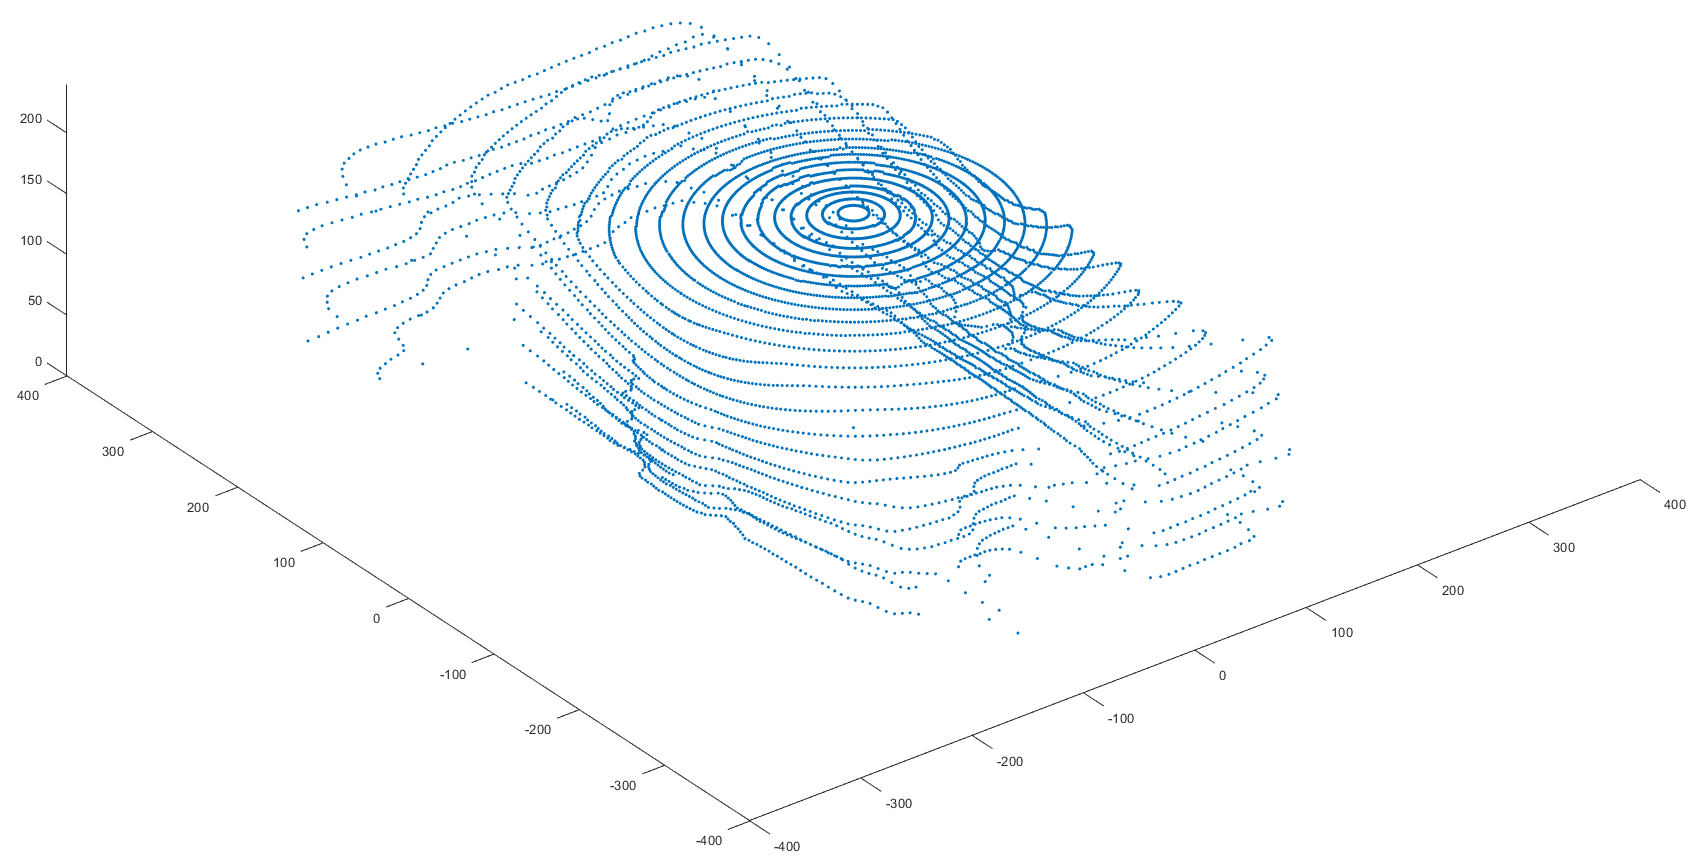
\includegraphics[width=0.9\textwidth]{images/Validierung/Aufloesungen/niedrig.png}
	\caption{Niedrige Auflösung}
	\label{niedrig}
\end{figure}


Bei der mittleren Auflösung werden etwa 16 mal so viele Bildpunkte aufgenommen wie bei der Messung mit geringer Auflösung. Die vertikale Schrittweite wird im verglich zur ersten Messung halbiert, die horizontale beträgt mit 0,15 Grad ein Achtel der ursprünglichen Schrittweite. 

Die horizontalen Punkte verschmelzen zu einer Linie. Dies ist ein Zeichen dafür, dass die horizontle Auflösung von 0,15 Grad für den Testraum vollkommen Ausreicht. Durch die geringere vertikale Schrittweite erhält man doppelt so viele Messebenen. Dadruch werden Details wie beispielsweise Türrahmen, Lampen und weitere Gegenstände besser erkennbar. 


\begin{figure}[H]
	\centering
	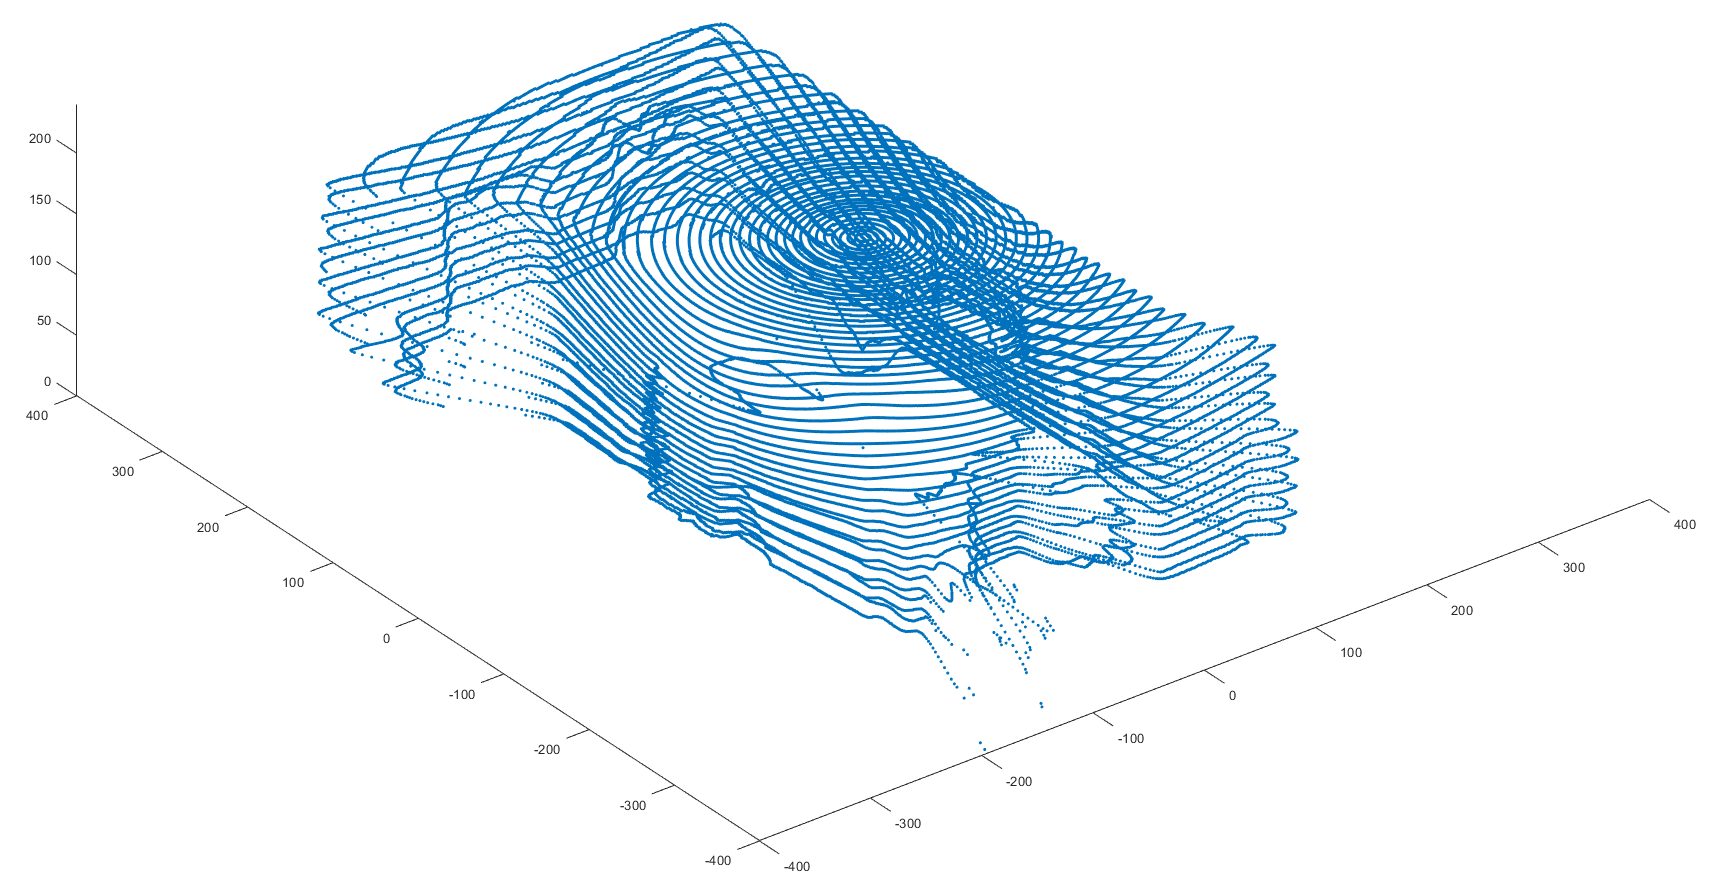
\includegraphics[width=0.9\textwidth]{images/Validierung/Aufloesungen/mittel.png}
	\caption{Mittlere Auflösung}
	\label{mittel}
\end{figure}

Wie die Messung mit mittlerer Auflösung bereits gezeigt hat, reicht eine horizontale Schrittweite von 0,15 Grad bei der Größe des Testraums aus. Für den Test mit hoher Auflösung wird daher nur noch die vertikale Schrittweite halbiert. Dadurch verdoppelt sich die Anzahl der Bildpunkte. Die Messung benötigt jedoch ungefährt doppelt so lange.

Das Ergebnis ist eine 3D-Aufnahme, bei der sowohl horizontale als auch vertikale Auflösung gut ausreicht, um Details erkennen zu können.

\begin{figure}[H]
	\centering
	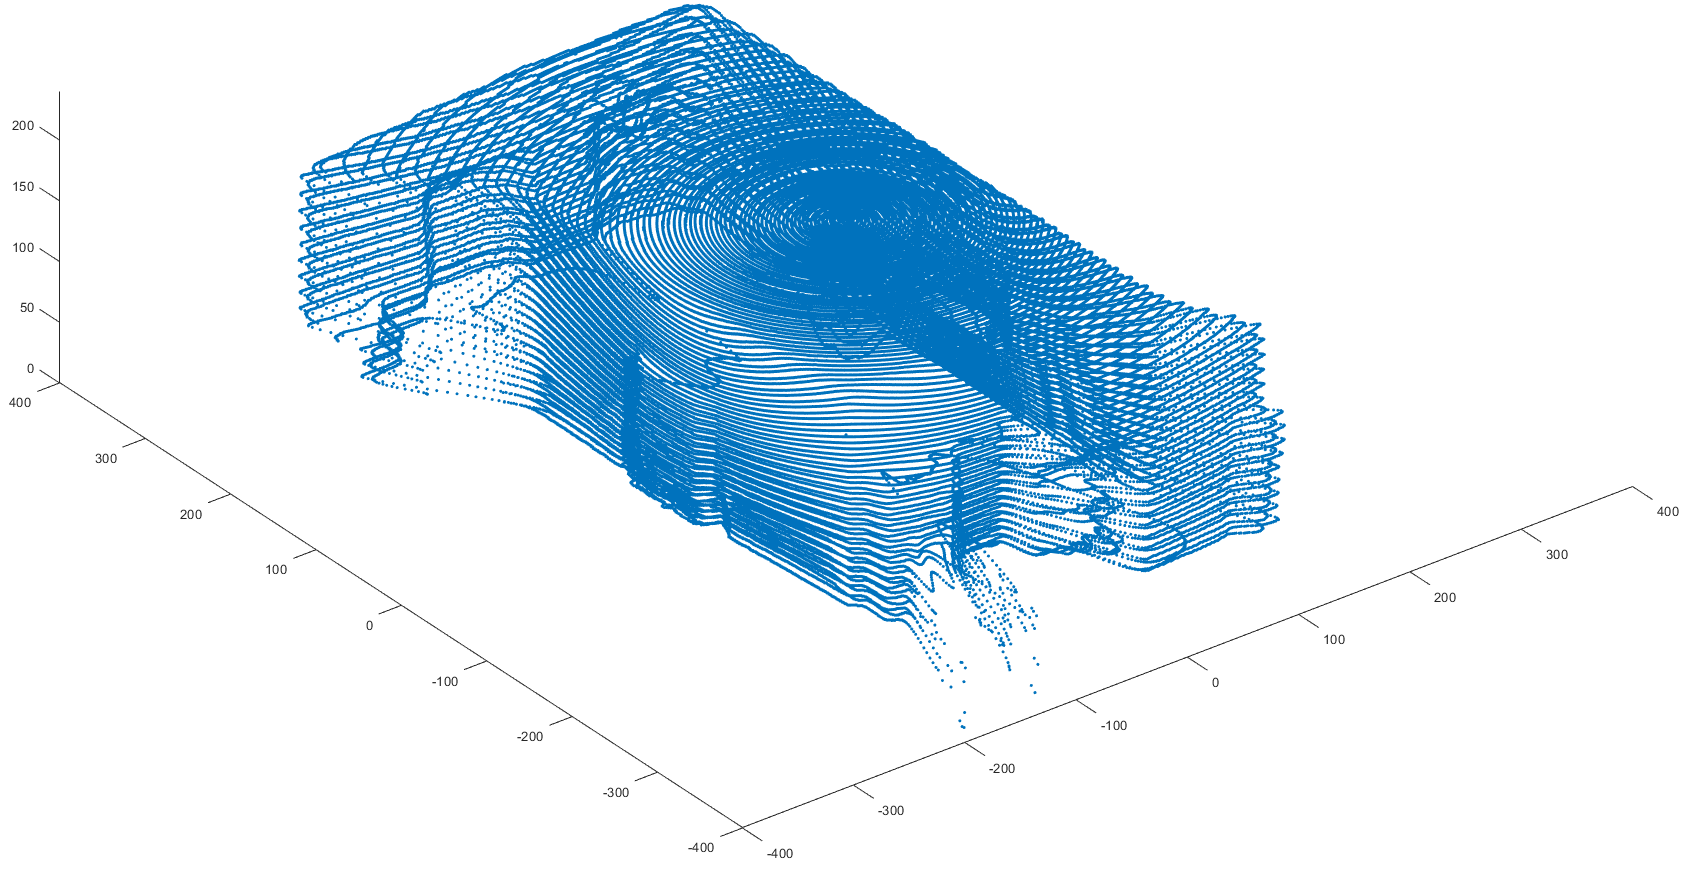
\includegraphics[width=0.9\textwidth]{images/Validierung/Aufloesungen/hoch.png}
	\caption{Hohe Auflösung}
	\label{hoch}
\end{figure}


Weiter werden die erstellten Grundrisse mit niedriger, mittlere und hoher Auflösung mit dem tatsächlichen Grundriss verglichen.

Der Vergleich zeigt, dass die Maße immer bis auch geringe Abweichungen mit dem tatsächlichen Grundriss übereinstimmten. Dabei macht die Auflösung keinen Unterschied. 

Deutlich erkennbar ist jedoch, wie in Bild .-- zu sehen, dass bei niedriger Auflösung Details wie Türrahmen verschwimmen. Zudem sind die einzelnen Linienebenen leicht zueinander verschoben und nicht eindeutig zuordenbar.
Im Vergleich dazu sind bei der hohen Auslösung klare Grundrisslinien erkennbar.


\begin{figure}[htb]
	\centering
	\begin{minipage}[t]{0.45\linewidth}
		\centering
		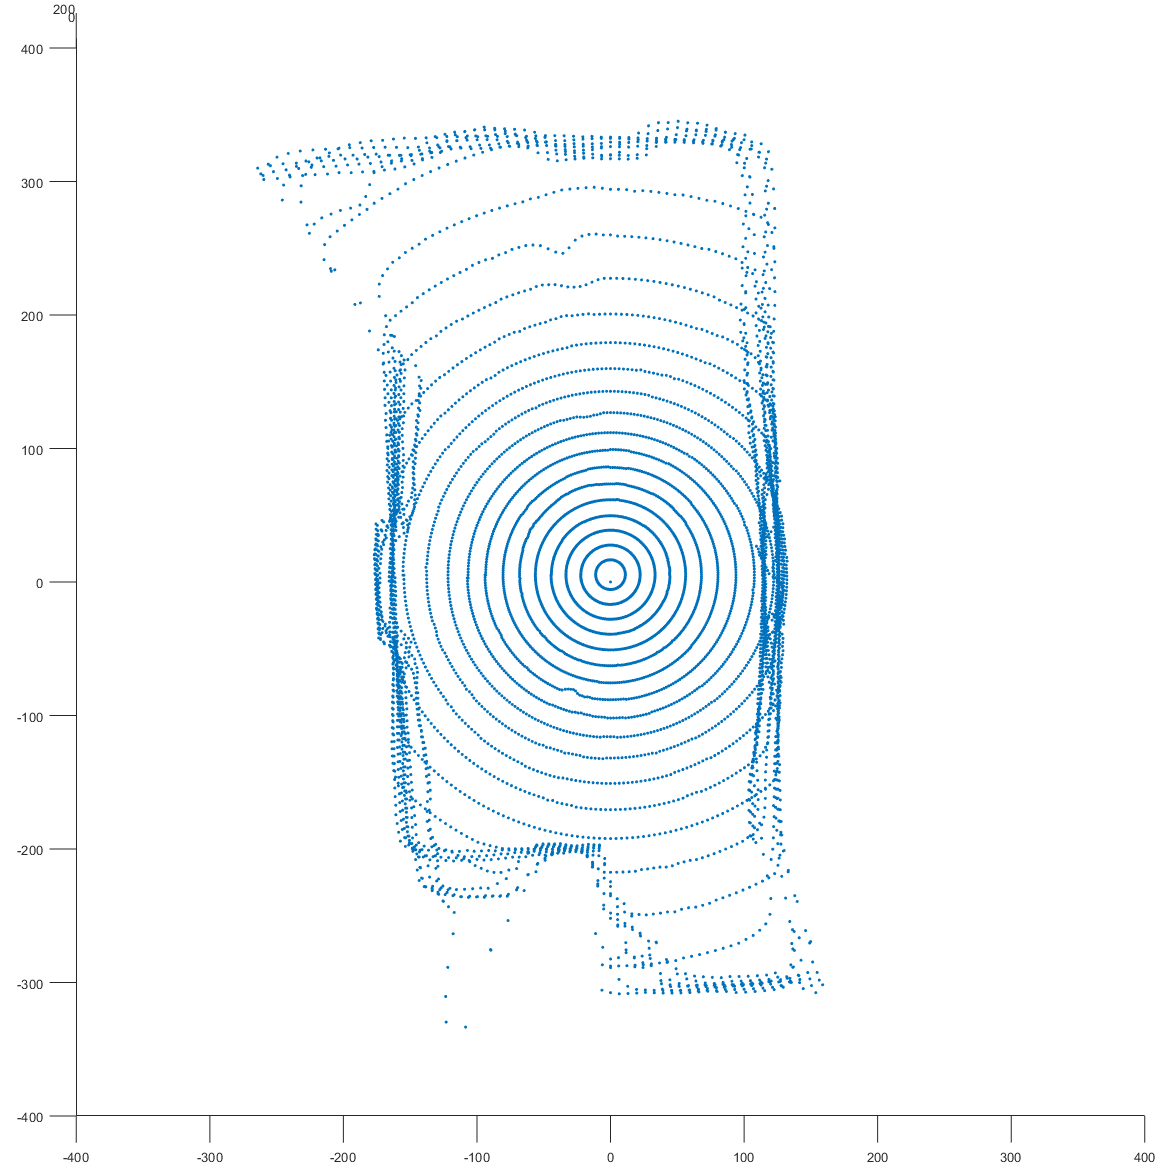
\includegraphics[width=1.2\linewidth]{images/Validierung/Aufloesungen/niedrig_vogel.png}
		\caption{Beispielbild}
	\end{minipage}
	\hfill
	\begin{minipage}[t]{0.45\linewidth}
		\centering
		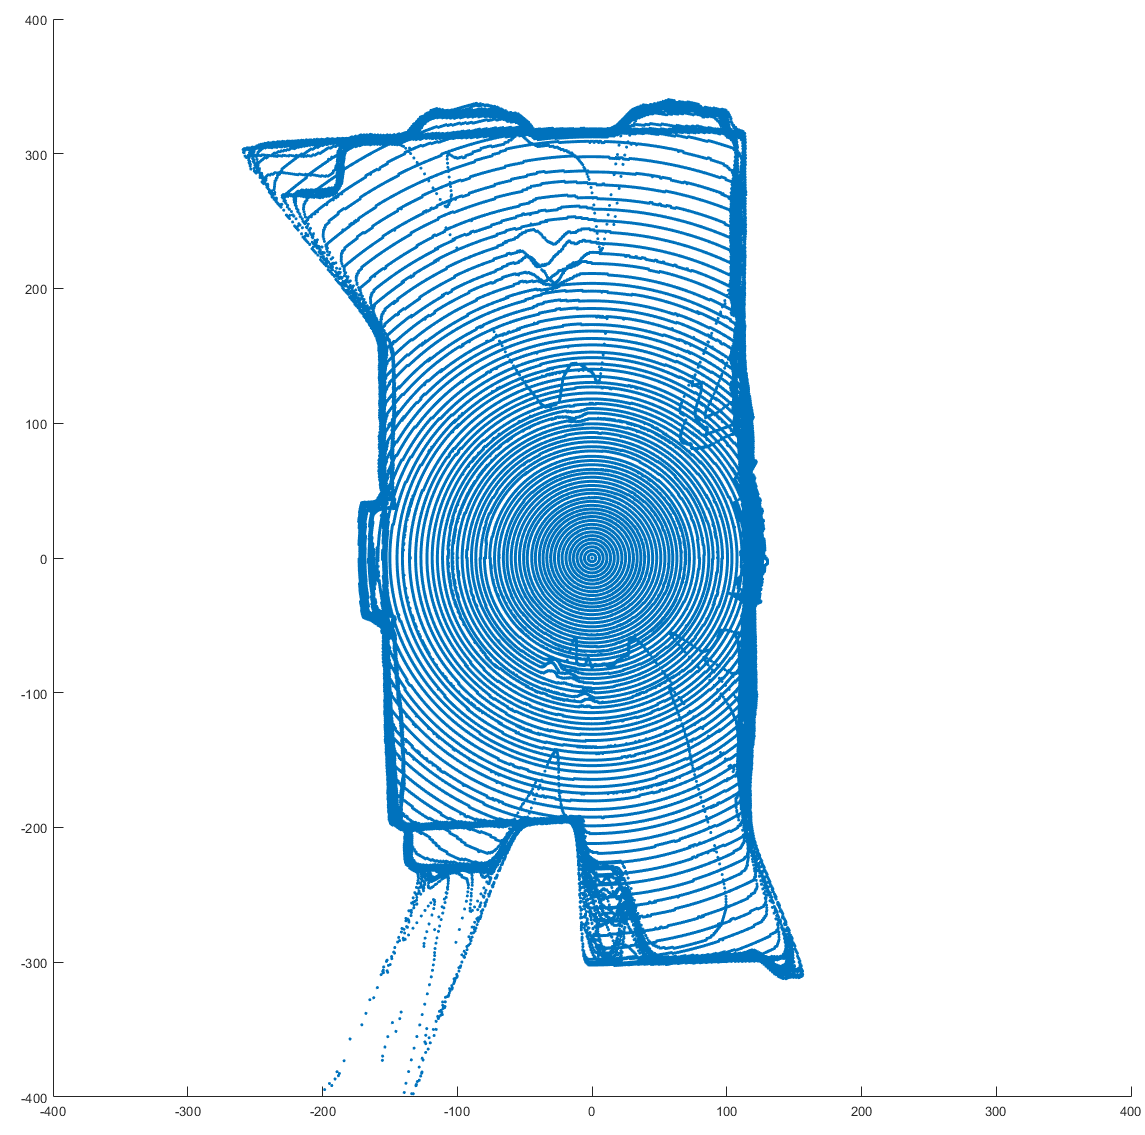
\includegraphics[width=1.2\linewidth]{images/Validierung/Aufloesungen/hoch_vogel.png}
		\caption{Beispielbild}
	\end{minipage}
\end{figure}


Im Großen und Ganzen lässt sich sagen, dass je nach Anforderung an das System die Parameter dementsprechend eingestellt werden müssen. Möchte man nur einen groben Überblick über den Raum, reicht ein schneller Scan mit niedriger Auflösung vollkommen aus. Möchte man hingegen eine detailreiche Darstellung, bei der man auch Details virtuell vermessen kann, wird die hohe Auflösung benötigt. Dafür dauert solch eine Messung im Vergleich zu schnellen Messung recht lange.
Man sollte somit immer einen Kompromiss zwischen benötigter Auflösung und der Zeit für die Messung finden.



\section{Vergleich der Sensoren}

Nachdem sowohl die Mechanik als auch der erste Lidar Sensor getestet und validiert wurden, soll ein kostengünstigerer Sensor getestet werden. Dazu werden zwei Aufnahmen mit den gleichen Einstellungen aber verschiedenen Sensoren Aufgenommen. Die erste Messung wird mit dem Sensor "TF MINI" gemacht. Als zweiter Sensor wird ... genommen.

 

\begin{figure}[H]
	\centering
	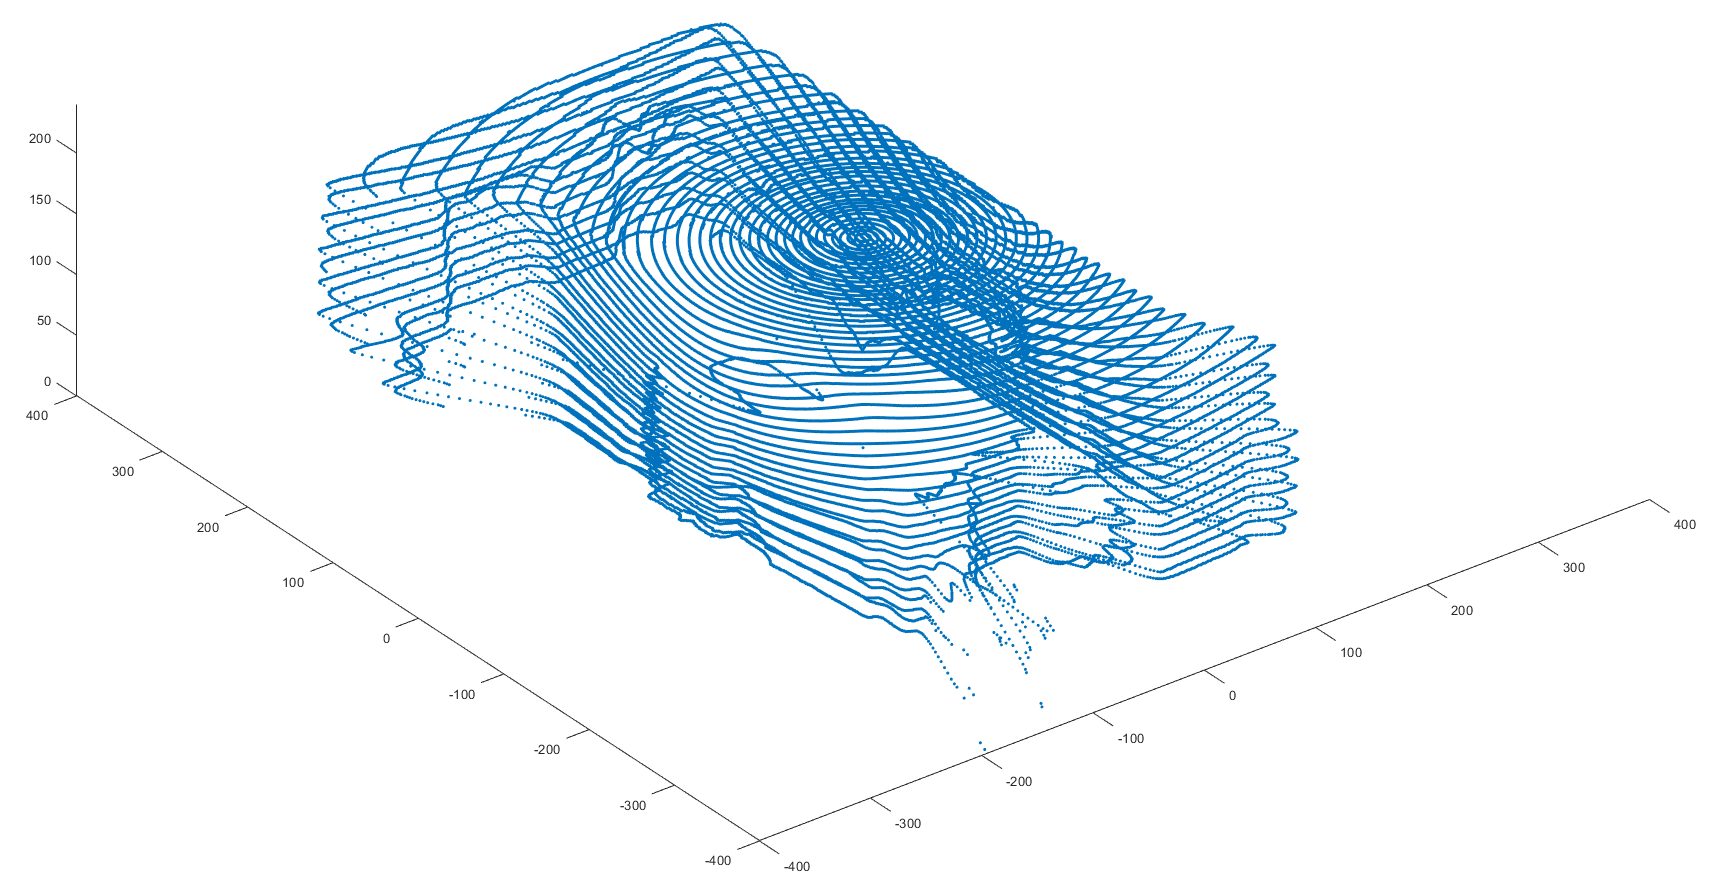
\includegraphics[width=0.9\textwidth]{images/Validierung/Aufloesungen/mittel.png}
	\caption{TF MINI}
	\label{hoch}
\end{figure}

\begin{figure}[H]
	\centering
	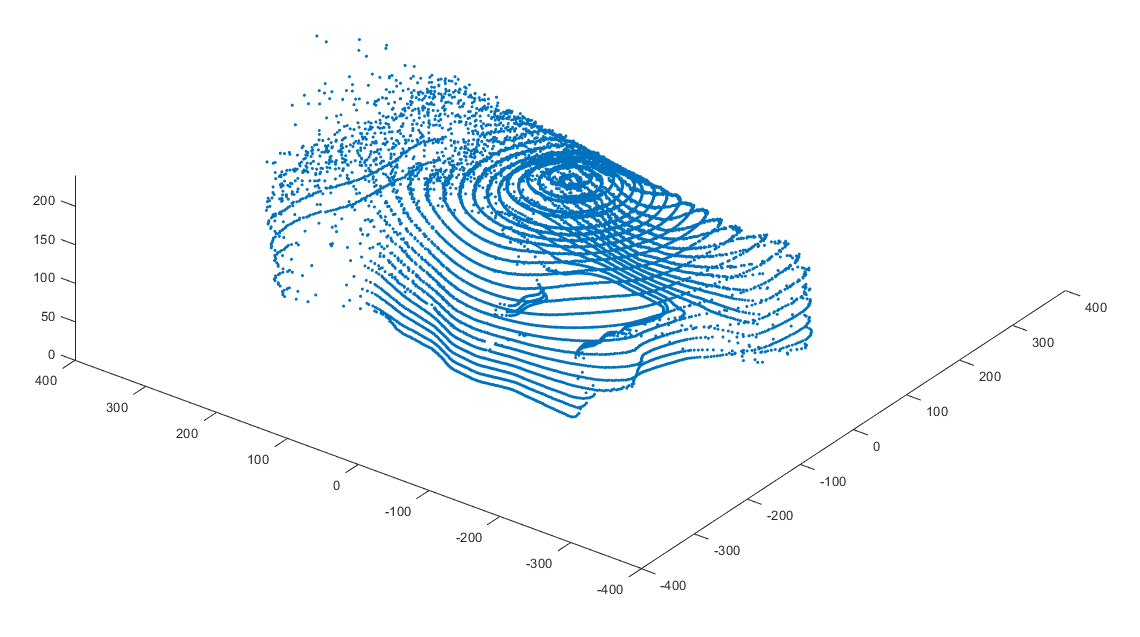
\includegraphics[width=0.9\textwidth]{images/Validierung/VLX_gerade.png}
	\caption{Sensor VLX}
	\label{vlx}
\end{figure}

\begin{figure}[H]
	\centering
	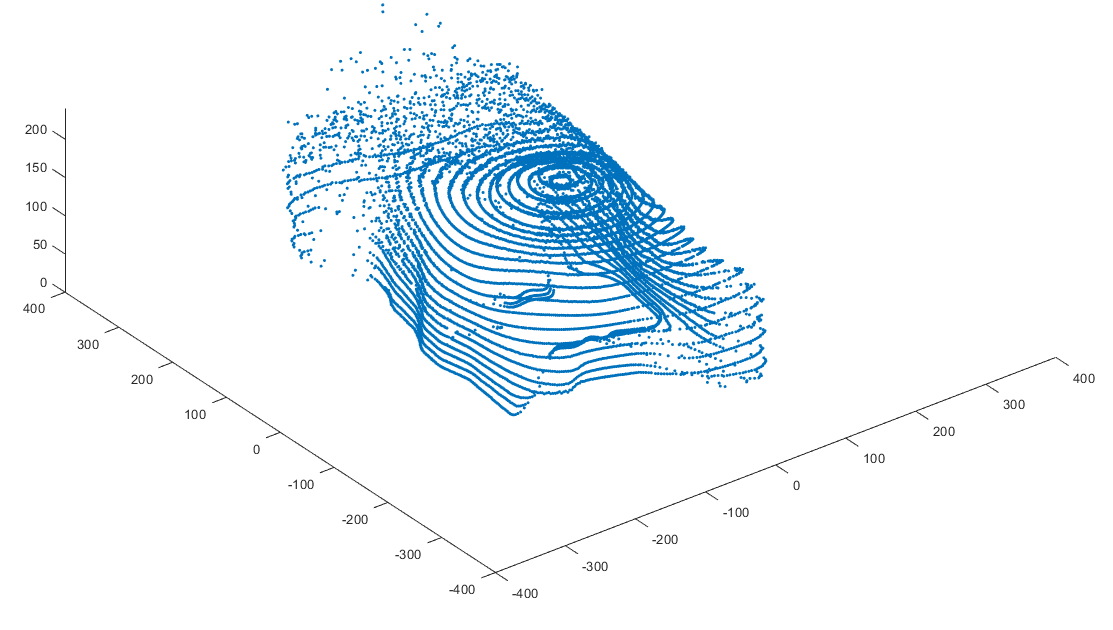
\includegraphics[width=0.9\textwidth]{images/Validierung/VLX.png}
	\caption{Sensor VLX}
	\label{vlxa}
\end{figure}



\begin{figure}[htb]
	\centering
	\begin{minipage}[t]{0.45\linewidth}
		\centering
		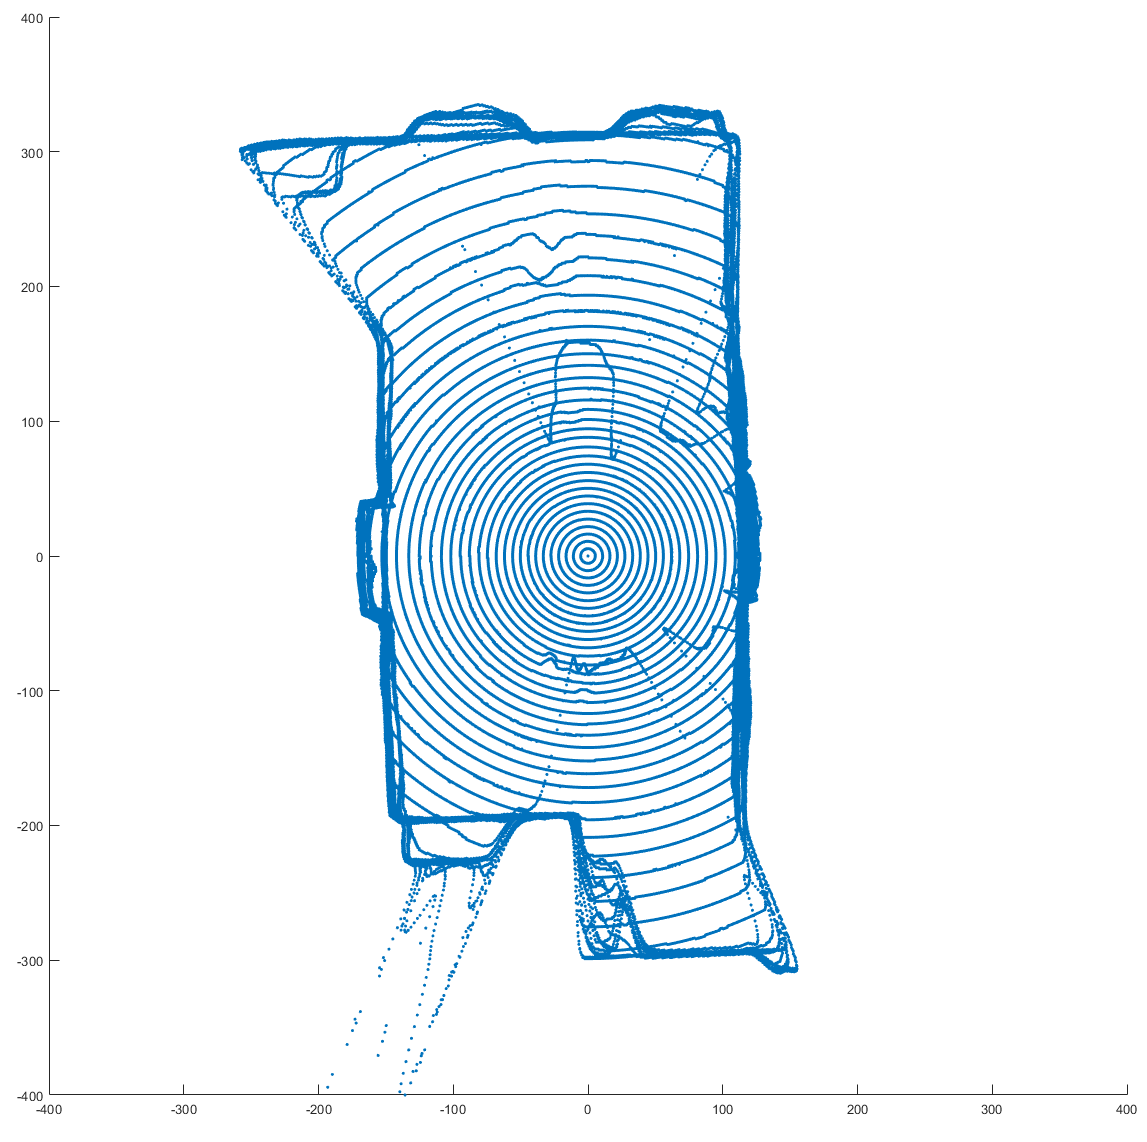
\includegraphics[width=1.2\linewidth]{images/Validierung/Aufloesungen/mittel_vogel.png}
		\caption{Beispielbild}
	\end{minipage}
	\hfill
	\begin{minipage}[t]{0.45\linewidth}
		\centering
		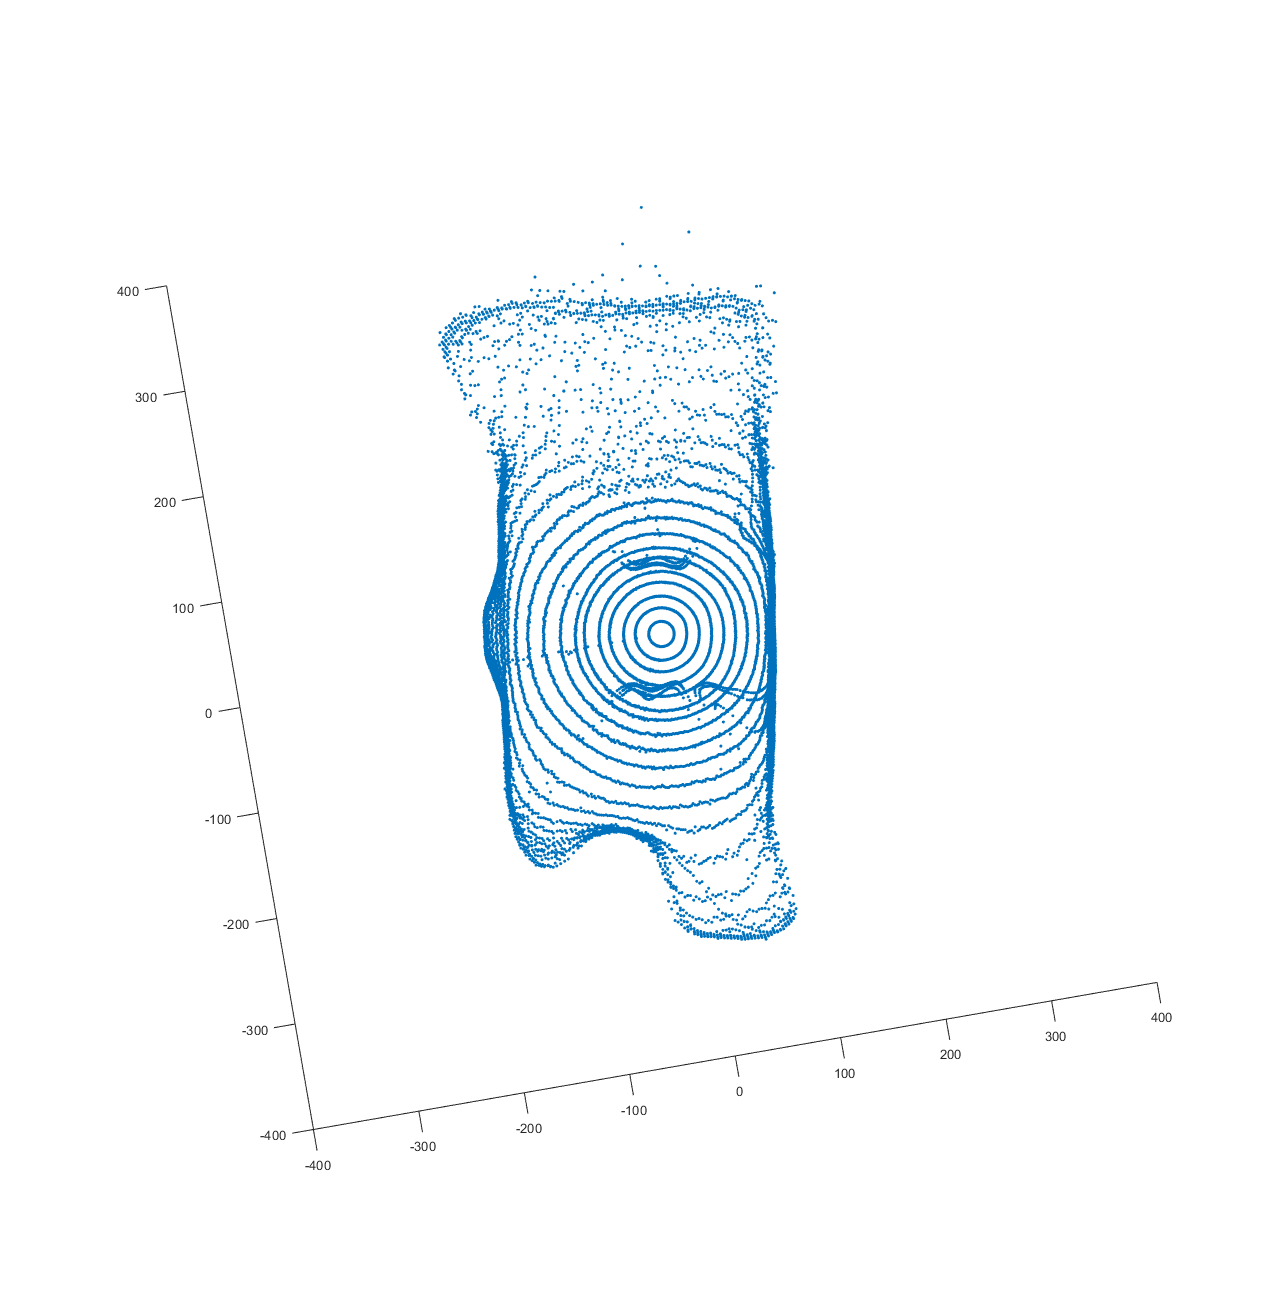
\includegraphics[width=1.2\linewidth]{images/Validierung/VLX_vogel.png}
		\caption{Beispielbild}
	\end{minipage}
\end{figure}







